\chapter{野中葉研究会ムスリム共生プロジェクト}
中澤仁研究室に加え, 私が参加していた慶應義塾大学総合政策学部教授野中葉博士が持つ研究会,
「野中葉研究会 ムスリム共生プロジェクト」の活動について述べる.
まずはじめに, Halal Guide Project について述べ, 次に私が作成した訪日・在日ムスリムむけ
webアプリケーション「Halal Checker」について述べる.
最後にまとめおよび野中葉研究会への謝辞を述べる.

\section{HalalGuideProject}
野中葉研究会ムスリム共生プロジェクトには4つのプロジェクトが存在する.(2020年1月28日現在)
「Welcome Muslim Friends」,「MUSLI-MAP PROJECT」, 「Nonakalab Channel」に加え,
私は「Halal Guide Project」に参加し, 訪日ムスリムにむけた情報提供型おもてなしを情報技術を使って
行った. 3年生の春学期より4年生春学期までプロジェクトリーダーを務めさせていただき,
プロジェクトの進行,発展のため活動をした.
次節では,4年時に作成した訪日・在日ムスリム向けアプリケーション「Halal Checker」について記述する.

\section{Halal Checker}
本節では訪日・在日ムスリム向けアプリケーション「Halal Checker」について述べる.
最初に概要を述べた後, 背景と現状日本にいるムスリムがかかえる問題点を挙げ, 本プロジェクトの目的および
アプローチを述べる. アプリケーションの実装を説明した後, 最後に今後の展望について述べる.
\subsection{概要}
本プロジェクトは, 訪日・在日外国人ムスリムへむけた食品ラベルから, イスラームの教えに反した成分を検出し,
日本語がわからないユーザーにピクトグラムによる情報開示を行うアプリケーションである.
年々増加傾向にあるムスリムが日本を快適に楽しむために,開発したアプリケーションである.

\subsection{背景・問題}
年々, 世界のムスリム人口は急激に増加している.現在は,世界人口の4人に1人がイスラーム教徒と言われており,
近い将来3人に1人がイスラーム教徒になると言われている.
イスラーム国家と言われる東南アジアのインドネシアとマレーシアからの訪日外国人が増加しており,
訪日イスラーム教徒が日本でも増加傾向にある.
\begin{figure}[htbp]
    \begin{center}
       \fbox{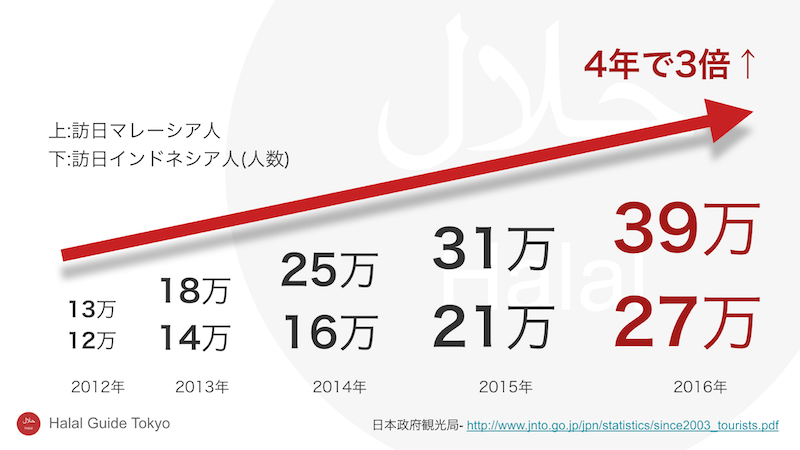
\includegraphics[width=150mm,bb=0 0 800 450]{muslimvistor.jpg}}
    \end{center}
    \caption{東南アジアからの訪日ムスリム数}
    \label{fig:muslimvistor}
\end{figure}
しかし, 訪日ムスリムを受け入れるための準備が日本ではまだ不十分である.
礼拝スペースの確保や, 外国語の表記など対応がまだまだ進んでいない.
その中でも, 食事に関してイスラームの教えに反する豚やアルコール成分が含まれる商品を
訪日・在日外国人ムスリムが自分で判別することは困難である.
特にコンビニエンスストアなど自身で食品ラベルを確認して,含まれる成分を判断することは
漢字表記など複雑にかかれているため外国人が解読するには難しい.

\subsection{目的・アプローチ}
本プロジェクトの目的は, 訪日・在日外国人ムスリムが日本で快適に過ごすために,
自身による食選択の判断を助長することである.
食品ラベルからイスラームの教えに反する食品成分を検出し, ムスリムのユーザーへ情報を開示する
システムの開発を行う.

\subsection{実装}
システム構成図を図\ref{fig:halal_checker_system}に示す.
食品ラベル画像を撮影し, 画像処理を行いOCR処理をgoogle cloud visionを用いて行う.
受け取った文字配列にイスラームの教えに反する文字列が含まれた場合, ムスリムユーザーへ成分が含まれる
ことをピクトグラムで表示する.

\begin{figure}[htbp]
    \begin{center}
       \fbox{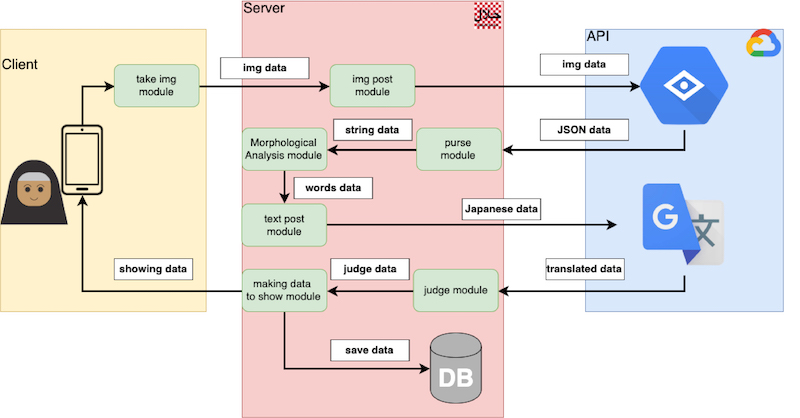
\includegraphics[width=150mm,bb=0 0 800 418]{halal_checker_system.jpg}}
    \end{center}
    \caption{Halal Checker システム構成図}
    \label{fig:halal_checker_system}
\end{figure}

\subsection{今後の展望}
今後はこのシステムを野中葉研究会のサーバー内の本番環境に設置し, 一般向けに公開をする.
また今後, 観光事業を行う企業との共同研究を行い, 実際に訪日ムスリムの目に届くところへ情報開示を行う予定である.

\section{まとめ}
増加するイスラーム教徒, そして訪日イスラーム教徒の増加に伴い日本社会において彼らとの共生は必要不可欠である.
日本で生活する彼らのために日本人としておもてなしをするツールの作成を行った.
今後, 私のイスラームを信仰する異国の友人たちが日本に訪れやすくなり, 日本社会ではマイノリティーであるイスラーム教徒の
方々が日本で生活する不安が少しでも緩和することを期待する.

\begin{figure}[htbp]
  \begin{minipage}{0.5\hsize}
    \begin{center}
       \fbox{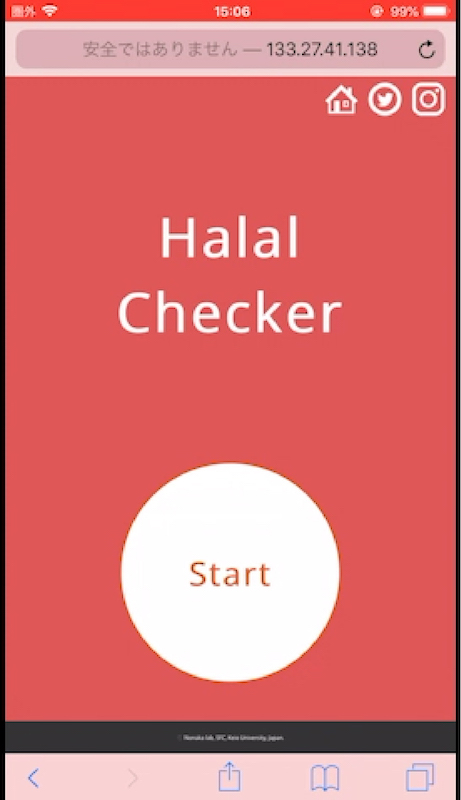
\includegraphics[width=60mm,bb=0 0 461 800]{hc_title.jpg}}
    \end{center}
    \caption{ユーザーインターフェース:タイトル}
    \label{fig:halal_checker_title}
  \end{minipage}
  \begin{minipage}{0.5\hsize}
    \begin{center}
       \fbox{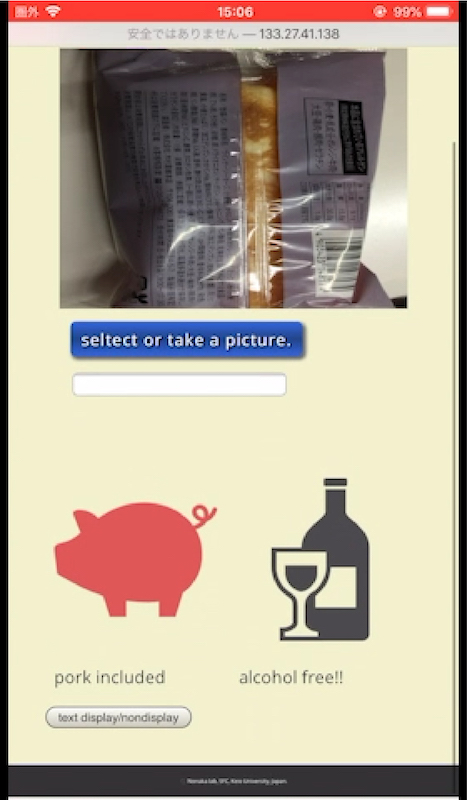
\includegraphics[width=60mm,bb=0 0 467 800]{hc_result.jpg}}
    \end{center}
    \caption{ユーザーインターフェース:結果画面}
    \label{fig:halal_checker_result}
  \end{minipage}
\end{figure}

\section{謝辞}
中澤仁研究室に所属しながらも, 研究室の1メンバーとして受け入れてくださった慶應義塾大学総合政策学部教授野中葉博士に深く感謝いたします.
また2年半の間,一緒に活動した野中葉研究会ムスリム共生プロジェクトメンバーへ深く感謝の意を表します.
そして,同じ研究室の中核として様々な助言をしていただいた,平松耕介氏,託見美由氏,栗原美優氏,土屋優介氏,徳山健輔氏,に深く感謝致します.
